\documentclass[10pt]{article}
\usepackage[letterpaper,margin=.7in]{geometry}
\usepackage[T1]{fontenc}
\usepackage{lmodern,graphicx,booktabs,longtable,array,hyperref,caption,float}
\hypersetup{colorlinks=true,urlcolor=blue,linkcolor=blue,pdftitle={Campi Flegrei: scientific progress and spending assessment}}
\setlength{\parindent}{0pt}
\setlength{\parskip}{5pt}
\setlength{\emergencystretch}{3em}
\captionsetup{font=small,labelfont=bf}
\newcommand{\file}[1]{\path{#1}}
\newcommand{\ev}[1]{\textsuperscript{[\hyperref[app:evidence]{#1}]}}
\begin{document}
\begin{center}
{\Large\bfseries Campi Flegrei: scientific progress and spending assessment}\par
\small Independent reproduction of Tan et al. (2025), \emph{Science} 390, 70--75\par
12 October 2026 $\mid$ Evidence assessed at commit \texttt{f115c20841779aac4c580327abe71e49499ae981}
\end{center}

\section*{Decision summary}
The project has recovered historical context and a limited waveform-processing capability, but not the paper's central earthquake-location results. Saved tables contain 90,017 picks, 908 provisional associations, and 53 conditional magnitudes; scientific accuracy remains unestablished. The principal obstacle is an unvalidated event/location foundation, compounded by sparse coverage and unverified velocity inputs. \textbf{Recommend one bounded, seismologist-led review of existing events, then stop unless it passes a predeclared credibility test.} Further open-ended agent development or multiyear processing is not presently justified. Past expenditure does not alter that decision.\ev{E1--E5}

\section*{Scientific accomplishments and their limits}
The strongest result is the displacement history (Figure~\ref{fig:gnss}): 8,743 daily GNSS observations through 20 March 2025 and 128 historical entries, including 14 source-derived estimates/reconstruction. It reaches 3.0504~m above its 1905 datum, subject to stitching assumptions. The external routine catalog contains 12,503 located study-period events, 420 (3.48\%) above the paper's 12,083, and five $M_d\geq4$ events. This recovers context, not independent earthquake detections.\ev{E2}

\begin{figure}[H]
\centering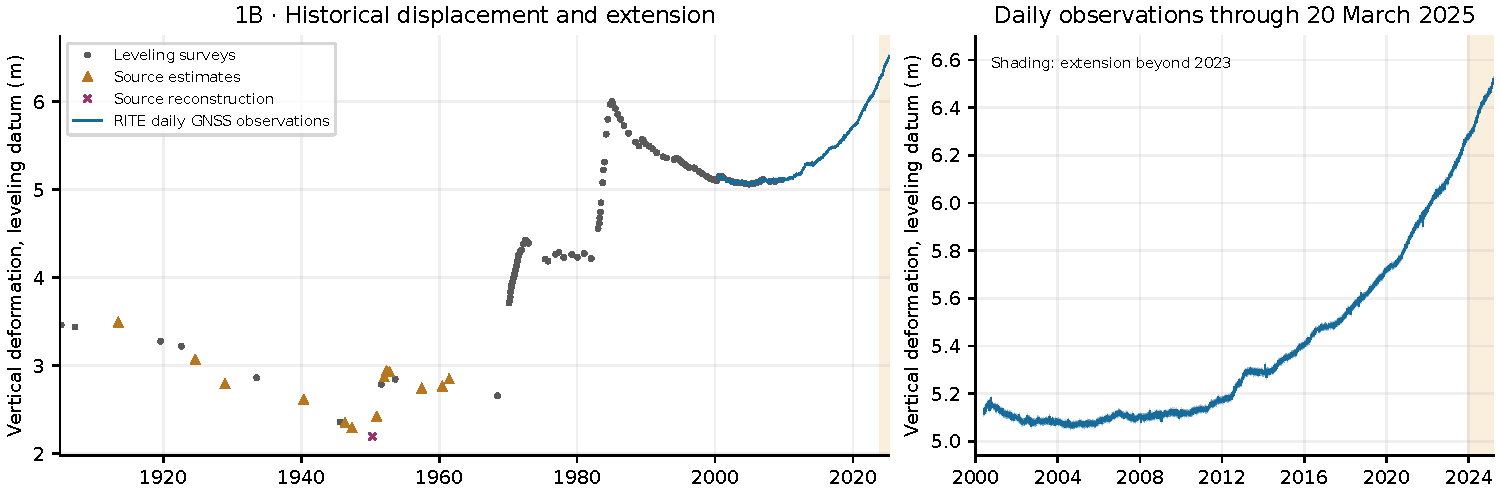
\includegraphics[width=\linewidth]{figures/figure_1B_displacement.pdf}
\caption{Existing Fig.~1B counterpart: surveys, source estimates/reconstruction, and GNSS are distinguished. The leveling datum equals 1905-relative displacement plus 3.464~m. Shading marks the extension beyond 2023. No image supplied these numbers.}\label{fig:gnss}
\end{figure}

\small
\begin{tabular}{p{.30\linewidth}p{.28\linewidth}p{.34\linewidth}}
\toprule
Published scientific finding & Existing independent evidence & Assessment \\
\midrule
54,319 final earthquakes; greater detection & 908 initial candidates; no accepted relocated catalog & Functioning pilot; detection gain untested \\
Narrow ring faults, 2.1--3.7~km depth; shallow northern faults & Initial depths 0--8~km; no validated relative locations & Geometry and depth limit untested \\
Slip mechanisms and absence of upward migration & No mechanisms; strongly uneven time coverage & Untested, not contradicted \\
70 hybrid events and their evolution & 822 unreviewed crossings; one corresponding waveform example & Example partly recovered; population/timing untested \\
\bottomrule
\end{tabular}
\normalsize

\clearpage
\section*{Coverage and location credibility}
\begin{figure}[H]
\centering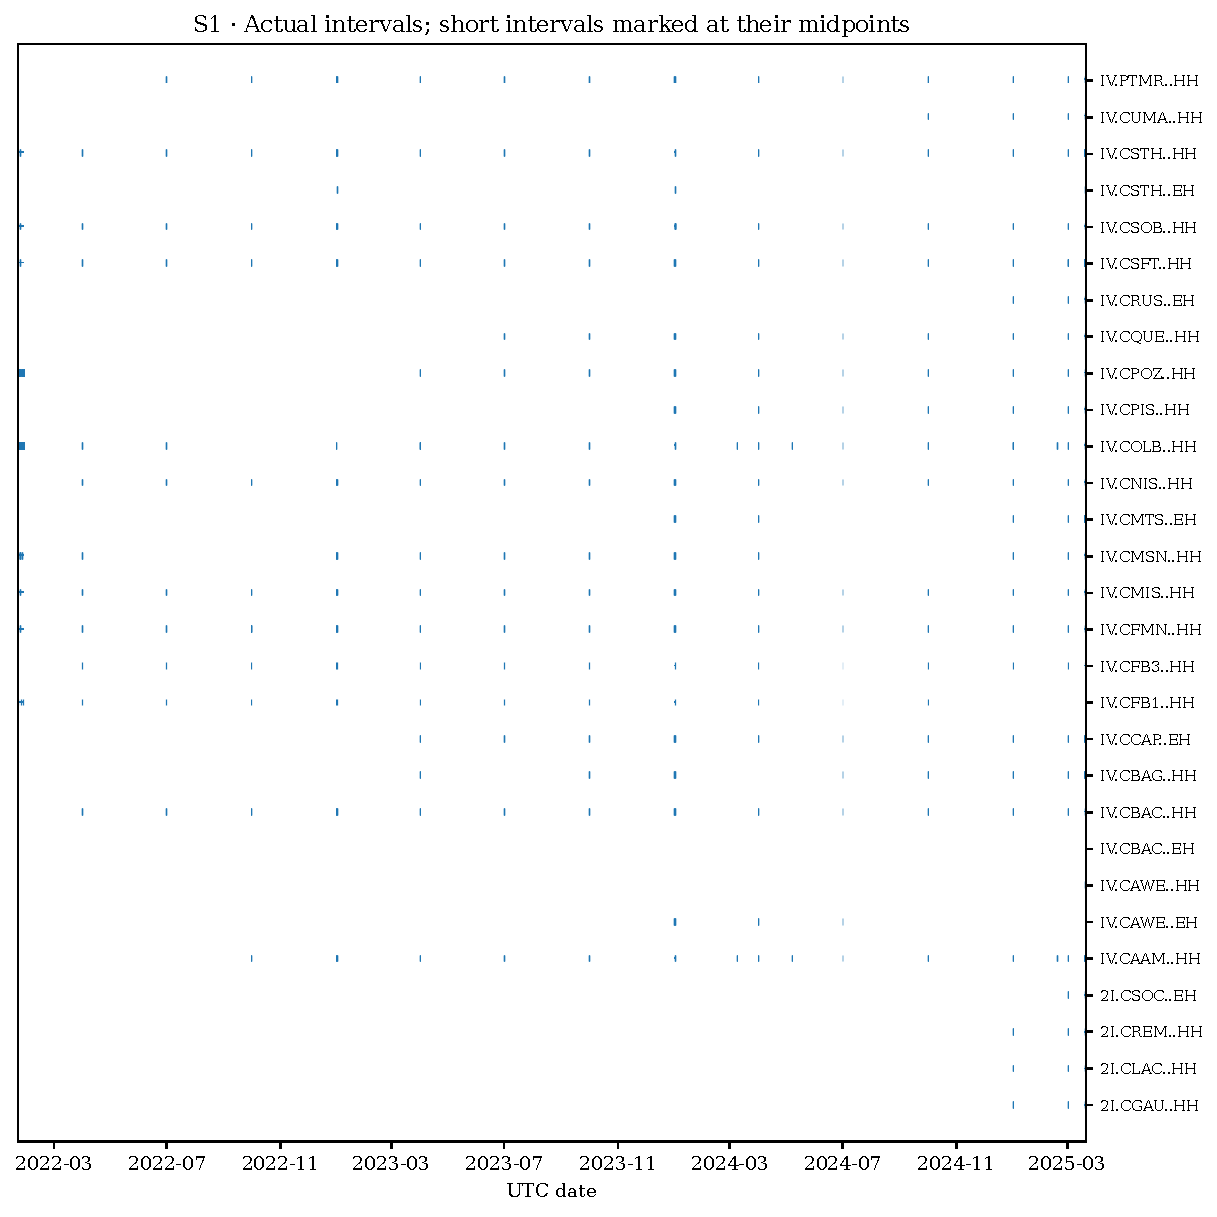
\includegraphics[width=.96\linewidth]{figures/continuation_coverage.pdf}
\caption{Existing generated S1 counterpart: actual processed station intervals, not requested coverage. Narrow marks include half-hour calendar samples. The multiyear axis conceals severe undersampling; 91.3\% of provisional events occur on 19--20 March 2025.}\label{fig:coverage}
\end{figure}

The saved interval union contains 4,278.694 channel-hours from 608 files, 83 channels and 26 station names, versus the paper's 48 instruments. All processed hours have response metadata; calibration accuracy is untested. Public INGV retrieval worked. Of the frozen queue, 434 requests succeeded, six returned no data and 74,234 remain pending; pending requests are unfinished acquisition, not inaccessible observations. RAN waveforms require credentials. Local archive examples are event-selected cuts and were excluded from independent detection.\ev{E1,E6}

\begin{center}\small
\begin{tabular}{lrr}
\toprule
Processing stage & Existing outputs & Paper's written totals \\
\midrule
P / S picks & 13,077 / 76,940 & 3,252,660 / 5,790,284 \\
Associated P / S picks & 1,756 / 4,770 & 632,601 / 765,808 \\
Initial associations & 908 & 105,944 \\
Accepted VELEST / TomoDD locations & 0 / 0 & 61,809 / 54,319 \\
\bottomrule
\end{tabular}
\end{center}

Unequal exposure prevents comparing detection efficiency. Of 908 candidates, 573 have six picks, 74 have only S picks, and 227 occupy depth bounds (196 at 0~km; 31 at 8~km). Fifty-seven of 1,405 paired arrivals have nonpositive S--P; residual RMS is 0.651~s. The 111 depths exceeding 3.7~km cannot contradict the published limit without validated locations/regions. Sixty-four CPOZ gathers lack sector/depth review.\ev{E1,E3}

\clearpage
\section*{Magnitude pilot, validation, and unresolved obstacles}
\begin{figure}[H]
\centering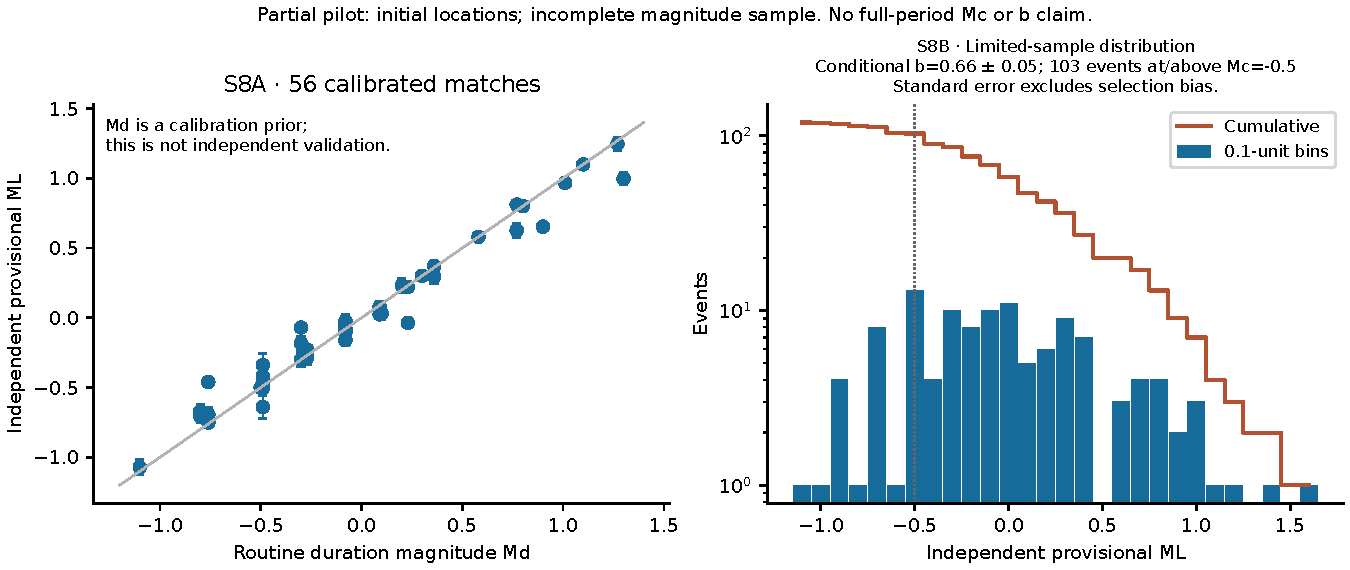
\includegraphics[width=\linewidth]{figures/figure_S8_pilot.pdf}
\caption{Existing partial S8 results. The 19 routine magnitudes on the left also anchor the inversion; proximity to the diagonal is not independent validation. The right panel contains only 53 selected magnitudes. Its apparent agreement with published completeness and $b$ is not a population-level reproduction.}\label{fig:mag}
\end{figure}

The implementation measured 60,092 channel amplitudes, retained 3,868 above 5~dB SNR, and formed 651 relative-amplitude equations. The 53 solved magnitudes span $-1.01$ to $1.94$. Maximum curvature gives $M_c=0.4$; only 21 events support $b=1.01\pm0.19$, versus the paper's 0.97. This formal error excludes selection and calibration bias. Hybrid scanning covers 75.797 common CAAM/COLB hours, with zero confirmed events; no three-year timing conclusion follows.\ev{E4,E5}

This assessment rechecked coverage, counts, exclusions, magnitude equations, 252 manifest hashes, and 11 panel chains; three waveform receipts/headers and both response files were spot-checked. Earlier analytical tests and 60 window-equivalence checks were inspected, not rerun. A 120-event alternative-profile VELEST experiment has equal saved velocities/depths across 32/64-bit runs, but four epicenters differ by up to 11.1~m; RMS is 0.389~s. Scientific location validation is absent. Numerical consistency is stronger than observational validation.\ev{E1,E3,E7}

\textbf{Obstacles ranked by scientific consequence:}
\begin{enumerate}\setlength{\itemsep}{0pt}
\item \textbf{Event/location validity and incomplete methods.} Manual review is missing. The exact 2018 starting profile is absent; the distributed 3D grid's transformations are unverified. The 2021 alternative, association settings, and unit magnitude-prior weight are explicit assumptions, not validated equivalents.
\item \textbf{Coverage and unfinished processing.} Most public retrieval remains unattempted. TomoDD rounds, S7 uncertainty, mechanisms, and hybrid validation/clustering are not completed; RAN access is an additional limitation.
\item \textbf{Provenance and implementation history.} Grid-dependent S6 results were withdrawn. A magnitude rerun changed the amplitude-table hash; the earlier table was not retained to resolve why. Downstream equations and magnitudes were unchanged. Historical source reconstructions are labeled; synthetic tests and published comparison images are excluded from inspected empirical chains.\ev{E6--E8}
\end{enumerate}

\clearpage
\section*{Value of additional spending}
Retrieval, inference, coverage accounting, and amplitude measurements are reusable if associated signals represent coherent earthquakes. More figure production cannot establish this. Model provenance requires institutional information; polarities and hybrid classification require scientific judgment. Bulk acquisition is processing work, not a reason for repeated agent reasoning.

\begin{table}[H]\small
\caption{One proposed next step; not authorized or executed.}
\begin{tabular}{p{.23\linewidth}p{.71\linewidth}}
\toprule
Scientific question & Are the provisional events sufficiently credible to justify a bounded location study? \\
Specific work & Predeclare 30 ordinary, depth-bound and S-only cases. A seismologist reviews original multistation waveforms, assignments and S--P consistency. No catalog-seeded selection or tuning; agent assembles evidence. \\
Deliverable & Thirty traceable reviews, confirmed/rejected/indeterminate counts, failure categories, and a spending decision. \\
Success criterion & At least 24/30 coherent multistation earthquakes; no unexplained invalid S--P among accepted events; judgments linked to observations. Proposed funding threshold, not published accuracy or unbiased catalog precision. \\
Agent estimate and ceiling & Range: 0.5--2 million input tokens (cached included), 5,000--20,000 output (reasoning included). Ceiling: 2 million input/20,000 output; no additional agents. \\
Data / computation / people & Existing observations only; no downloads. At most one CPU-hour for small read/display checks, no full rerun. At most four seismologist-hours; human review is required. \\
Principal risk / stop & False associations or inadequate waveforms. Stop at any ceiling or indeterminate/failed test. Passing permits a location-validation proposal, not full-period processing. \\
\bottomrule
\end{tabular}
\end{table}

These uncertain allowances cover one review set/evidence package, without algorithm development; they are not measured forecasts. Prior session counters record 128.58 million input tokens (125.04 million cached) and 0.891 million output tokens. These are session totals, not audited billing. Account rates and project billing are unavailable; dollar estimates are unjustified. Logged successful stages took 3,589~s, excluding failures/downloads, and do not price a multiyear run.\ev{E9}

\textbf{Spending decision: approve only the bounded review if a seismologist can perform it; otherwise stop.} Do not authorize further development, bulk retrieval, or figure completion now. Even a successful review leaves exact velocity-model provenance and representative temporal coverage unresolved. The expected return is a credible decision about the event foundation, rather than another larger provisional catalog.

\small
\textbf{Scope.} Only inexpensive checks were run; earlier deliverables remain unchanged. The appendix inventories every panel. Central structural/mechanistic findings remain untested.\normalsize

\clearpage
\appendix
\section*{Appendix A: panel inventory}
\label{app:panels}
The inventory follows the captioned main panels and supplemental panels/views in \file{tanmodel.pdf} and \file{tanmodelsupp.pdf}: 10 main and 53 supplementary entries, 63 total. Composite waveform/score/spectrogram axes remain under their original lettered panel; unlettered spatial views and four S14 waveform groups are explicit. The S7A map and depth view are separate. Feature labels A--D in S9 are not additional panels. No inventory entry is a conceptual-only schematic. Tables S1--S2 and Data S1--S3/interactive S1 are accounted for below but are not added to the 63-panel denominator.

\textbf{Generation and agreement are separate.} P = partial independent processing of observations/metadata; C = calculation from expressly permitted external context/calibration; N = no valid current counterpart. ``Partial'' never means quantitative reproduction. Eleven entries have saved partial counterparts; 52 do not. None establishes full independent reproduction. Missing numerical agreement is stated rather than inferred from visual similarity. The following file aliases are repository-relative: D = \file{data/continuation/}; F = \file{figures/}; O = \file{data/observations/}. Chain labels C1--C8 are expanded after the inventory. All file links were checked locally. Ignored original inputs remain local and have retrieval receipts.
\begingroup\footnotesize\setlength{\tabcolsep}{4pt}
\begin{longtable}{p{.20\linewidth}p{.29\linewidth}p{.18\linewidth}p{.26\linewidth}}
\toprule Panel / quantity & Generation; data and plot evidence & Agreement & Principal limitation \\
\midrule\endfirsthead
\toprule Panel / quantity & Generation; data and plot evidence & Agreement & Principal limitation \\
\midrule\endhead
\bottomrule\endfoot
1A\newline INGV event map and large-event markers & \textbf{C}; C1. \path{D/figure_1A.csv}; \path{F/figure_1A_routine.pdf} & Five $M_d\geq4$ events agree with text; 16,046 mapped entries. & Different routine-catalog vintage; relief/zero contour absent; eight entries outside extent.\\[4pt]
1B\newline Vertical displacement at Pozzuoli port & \textbf{C}; C2. \path{D/rite_gnss.csv}; \path{D/historical_leveling.csv}; \path{F/figure_1B_displacement.pdf} & Historical pattern only; no error metric against paper. & Datum/benchmark assumptions; 14 source-derived historical entries; 319 daily gaps.\\[4pt]
1C\newline Temporal seismicity and cumulative counts & \textbf{C}; C1. \path{D/figure_1C.csv}; \path{D/figure_1C_cumulative.csv}; \path{F/figure_1C_routine.pdf} & 7,218 cumulative $M_d>0.2$; no matched-vintage error metric. & External snapshot differs; March 2025 is partial; not independent detections.\\[4pt]
2A\newline Catalog seismicity rates by region & \textbf{N}; C8. No valid current data/plot. & Not assessed. & No accepted relocated multiyear catalog; coverage and location validation incomplete.\\[4pt]
2B\newline Depth versus time, symbol size by magnitude & \textbf{N}; C8. No valid current data/plot. & Not assessed. & No accepted relocated multiyear catalog; coverage and location validation incomplete.\\[4pt]
3/map\newline Epicentral spatial pattern & \textbf{N}; C8. No valid current data/plot. & Not assessed. & No accepted relocated multiyear catalog; coverage and location validation incomplete.\\[4pt]
3/northing-depth\newline Depth versus northing & \textbf{N}; C8. No valid current data/plot. & Not assessed. & No accepted relocated multiyear catalog; coverage and location validation incomplete.\\[4pt]
3/easting-depth\newline Depth versus easting & \textbf{N}; C8. No valid current data/plot. & Not assessed. & No accepted relocated multiyear catalog; coverage and location validation incomplete.\\[4pt]
4A\newline Ring-sector focal mechanisms and seismicity & \textbf{N}; C8. No valid current data/plot. & Not assessed. & No reviewed polarities/ratios, accepted model, Green functions or SKHASH/gCAP solutions.\\[4pt]
4B\newline Central/onshore focal mechanisms and seismicity & \textbf{N}; C8. No valid current data/plot. & Not assessed. & No reviewed polarities/ratios, accepted model, Green functions or SKHASH/gCAP solutions.\\[4pt]
S1\newline Station data-availability timeline & \textbf{P}; C3. \path{D/processed_coverage_union.json}; \path{F/continuation_coverage.pdf} & 4,278.694 channel-hours; incomplete study period. & 608 files, 26 names; most continuous requests pending. Not deployment availability.\\[4pt]
S2\newline Station map & \textbf{P}; C4. \path{D/figure_S2.csv}; \path{D/station_geometry_qa.csv}; \path{D/station_geometry_epochs.csv}; \path{F/continuation_stations.pdf} & 51 candidates, 42 verified; paper uses 48 instruments. & Nine unresolved; aliases/membership unverified. All 51 retained and labeled.\\[4pt]
S3A\newline Noise example: waveform, phase labels, spectrogram & \textbf{N}; C8. No valid current data/plot. & Not assessed. & No independent retraining/annotations; exact examples absent. S3C/D are training augmentation, not empirical multi-event results.\\[4pt]
S3B\newline Single-event example: waveform, phase labels, spectrogram & \textbf{N}; C8. No valid current data/plot. & Not assessed. & No independent retraining/annotations; exact examples absent. S3C/D are training augmentation, not empirical multi-event results.\\[4pt]
S3C\newline Two overlapping events: waveform, phase labels, spectrogram & \textbf{N}; C8. No valid current data/plot. & Not assessed. & No independent retraining/annotations; exact examples absent. S3C/D are training augmentation, not empirical multi-event results.\\[4pt]
S3D\newline Five overlapping copies of one event: waveform, phase labels, spectrogram & \textbf{N}; C8. No valid current data/plot. & Not assessed. & No independent retraining/annotations; exact examples absent. S3C/D are training augmentation, not empirical multi-event results.\\[4pt]
S4A\newline Swarms at CSOB: waveform, spectrogram, original and retrained picker scores & \textbf{N}; C7. Related diagnostic only: \path{F/picker_comparison_CSOB.pdf} & Not assessed. & Different example windows; reference annotations and published benchmark not reproduced.\\[4pt]
S4B\newline CMIS noise: waveform, spectrogram, original and retrained picker scores & \textbf{N}; C7. Related diagnostic only: \path{F/picker_comparison_CMIS.pdf} & Not assessed. & Different example windows; reference annotations and published benchmark not reproduced.\\[4pt]
S5/map\newline Routine-catalog map & \textbf{C}; C1. \path{D/figure_S5.csv}; \path{F/figure_S5_routine.pdf} & 12,503 versus 12,083; +420 (+3.48\%). & Revised external routine catalog, not independent detections; exact snapshot absent. Three entries outside view.\\[4pt]
S5/northing-depth\newline Routine-catalog northing-depth & \textbf{C}; C1. \path{D/figure_S5.csv}; \path{F/figure_S5_routine.pdf} & 12,503 versus 12,083; +420 (+3.48\%). & Revised external routine catalog, not independent detections; exact snapshot absent. Three entries outside view.\\[4pt]
S5/easting-depth\newline Routine-catalog easting-depth & \textbf{C}; C1. \path{D/figure_S5.csv}; \path{F/figure_S5_routine.pdf} & 12,503 versus 12,083; +420 (+3.48\%). & Revised external routine catalog, not independent detections; exact snapshot absent.\\[4pt]
S6/map\newline Initial-location map & \textbf{N}; C8. Withdrawn; \path{quarantine/unverified_background/}; exploratory files in E3. & Not assessed. & Unverified 3D-grid origin; regional fit rejected. Alternative precision test is not S6.\\[4pt]
S6/northing-depth\newline Initial-location northing-depth & \textbf{N}; C8. Withdrawn; \path{quarantine/unverified_background/}; exploratory files in E3. & Not assessed. & Unverified 3D-grid origin; regional fit rejected. Alternative precision test is not S6.\\[4pt]
S6/easting-depth\newline Initial-location easting-depth & \textbf{N}; C8. Withdrawn; \path{quarantine/unverified_background/}; exploratory files in E3. & Not assessed. & Unverified 3D-grid origin; regional fit rejected. Alternative precision test is not S6.\\[4pt]
S7A/map\newline HypoDD locations and errors; map & \textbf{N}; C8. No valid current data/plot. & Not assessed. & No relocated regional subsets or HypoDD SVD; published typical ~10 m errors untested.\\[4pt]
S7A/easting-depth\newline HypoDD locations and errors; easting-depth & \textbf{N}; C8. No valid current data/plot. & Not assessed. & No relocated regional subsets or HypoDD SVD; published typical ~10 m errors untested.\\[4pt]
S7B\newline EX uncertainty versus differential-pick count & \textbf{N}; C8. No valid current data/plot. & Not assessed. & No relocated regional subsets or HypoDD SVD; published typical ~10 m errors untested.\\[4pt]
S7D\newline EY uncertainty versus differential-pick count & \textbf{N}; C8. No valid current data/plot. & Not assessed. & No relocated regional subsets or HypoDD SVD; published typical ~10 m errors untested.\\[4pt]
S7F\newline EZ uncertainty versus differential-pick count & \textbf{N}; C8. No valid current data/plot. & Not assessed. & No relocated regional subsets or HypoDD SVD; published typical ~10 m errors untested.\\[4pt]
S7C\newline EX uncertainty density by cluster & \textbf{N}; C8. No valid current data/plot. & Not assessed. & No relocated regional subsets or HypoDD SVD; published typical ~10 m errors untested.\\[4pt]
S7E\newline EY uncertainty density by cluster & \textbf{N}; C8. No valid current data/plot. & Not assessed. & No relocated regional subsets or HypoDD SVD; published typical ~10 m errors untested.\\[4pt]
S7G\newline EZ uncertainty density by cluster & \textbf{N}; C8. No valid current data/plot. & Not assessed. & No relocated regional subsets or HypoDD SVD; published typical ~10 m errors untested.\\[4pt]
S8A\newline Estimated local versus routine duration magnitude & \textbf{P}; C5. \path{D/figure_S8A.csv}; \path{F/figure_S8_pilot.pdf} & 19 calibration matches; no held-out accuracy test. & Same routine magnitudes regularize solution; provisional locations and prior weight.\\[4pt]
S8B\newline Magnitude-frequency distribution and fitted b value & \textbf{P}; C5. \path{D/figure_S8B.csv}; \path{D/magnitude_statistics.json}; \path{F/figure_S8_pilot.pdf} & $M_c=0.4$; $b=1.01\pm0.19$ vs 0.97, not population agreement. & 53 selected magnitudes; only 21 above threshold; selection bias not in error.\\[4pt]
S9/map\newline Filtered-catalog spatial views and feature labels A-D; map & \textbf{N}; C8. No valid current data/plot. & Not assessed. & No differential-time counts or relocated catalog for NCCP+NCCS>100 filter.\\[4pt]
S9/northing-depth\newline Filtered-catalog spatial views and feature labels A-D; northing-depth & \textbf{N}; C8. No valid current data/plot. & Not assessed. & No differential-time counts or relocated catalog for NCCP+NCCS>100 filter.\\[4pt]
S9/easting-depth\newline Filtered-catalog spatial views and feature labels A-D; easting-depth & \textbf{N}; C8. No valid current data/plot. & Not assessed. & No differential-time counts or relocated catalog for NCCP+NCCS>100 filter.\\[4pt]
S10/2022\newline Annual seismicity map & \textbf{N}; C8. No valid current data/plot. & Not assessed. & No accepted relocated multiyear catalog; coverage and location validation incomplete.\\[4pt]
S10/2023\newline Annual seismicity map & \textbf{N}; C8. No valid current data/plot. & Not assessed. & No accepted relocated multiyear catalog; coverage and location validation incomplete.\\[4pt]
S10/2024\newline Annual seismicity map & \textbf{N}; C8. No valid current data/plot. & Not assessed. & No accepted relocated multiyear catalog; coverage and location validation incomplete.\\[4pt]
S10/2025\newline Annual seismicity map & \textbf{N}; C8. No valid current data/plot. & Not assessed. & No accepted relocated multiyear catalog; coverage and location validation incomplete.\\[4pt]
S11/swarm-1\newline Map of one of four major swarms & \textbf{N}; C8. No valid current data/plot. & Not assessed. & No accepted relocated multiyear catalog; coverage and location validation incomplete.\\[4pt]
S11/swarm-2\newline Map of one of four major swarms & \textbf{N}; C8. No valid current data/plot. & Not assessed. & No accepted relocated multiyear catalog; coverage and location validation incomplete.\\[4pt]
S11/swarm-3\newline Map of one of four major swarms & \textbf{N}; C8. No valid current data/plot. & Not assessed. & No accepted relocated multiyear catalog; coverage and location validation incomplete.\\[4pt]
S11/swarm-4\newline Map of one of four major swarms & \textbf{N}; C8. No valid current data/plot. & Not assessed. & No accepted relocated multiyear catalog; coverage and location validation incomplete.\\[4pt]
S12A\newline Ring-sector division & \textbf{N}; C7. Related only: \path{D/cpoz_gathers.npz}; \path{F/cpoz_gather_diagnostic.pdf} & Not assessed. & 64 P-aligned gathers lack valid sector locations and deep-event review; not these panels.\\[4pt]
S12B\newline Ring-sector division in complementary spatial view & \textbf{N}; C7. Related only: \path{D/cpoz_gathers.npz}; \path{F/cpoz_gather_diagnostic.pdf} & Not assessed. & 64 P-aligned gathers lack valid sector locations and deep-event review; not these panels.\\[4pt]
S12C\newline Common-receiver gather: east / HHZ & \textbf{N}; C7. Related only: \path{D/cpoz_gathers.npz}; \path{F/cpoz_gather_diagnostic.pdf} & Not assessed. & 64 P-aligned gathers lack valid sector locations and deep-event review; not these panels.\\[4pt]
S12D\newline Common-receiver gather: southwest / HHZ & \textbf{N}; C7. Related only: \path{D/cpoz_gathers.npz}; \path{F/cpoz_gather_diagnostic.pdf} & Not assessed. & 64 P-aligned gathers lack valid sector locations and deep-event review; not these panels.\\[4pt]
S12E\newline Common-receiver gather: north / HHZ & \textbf{N}; C7. Related only: \path{D/cpoz_gathers.npz}; \path{F/cpoz_gather_diagnostic.pdf} & Not assessed. & 64 P-aligned gathers lack valid sector locations and deep-event review; not these panels.\\[4pt]
S12F\newline Common-receiver gather: east / HHN & \textbf{N}; C7. Related only: \path{D/cpoz_gathers.npz}; \path{F/cpoz_gather_diagnostic.pdf} & Not assessed. & 64 P-aligned gathers lack valid sector locations and deep-event review; not these panels.\\[4pt]
S12G\newline Common-receiver gather: southwest / HHN & \textbf{N}; C7. Related only: \path{D/cpoz_gathers.npz}; \path{F/cpoz_gather_diagnostic.pdf} & Not assessed. & 64 P-aligned gathers lack valid sector locations and deep-event review; not these panels.\\[4pt]
S12H\newline Common-receiver gather: north / HHN & \textbf{N}; C7. Related only: \path{D/cpoz_gathers.npz}; \path{F/cpoz_gather_diagnostic.pdf} & Not assessed. & 64 P-aligned gathers lack valid sector locations and deep-event review; not these panels.\\[4pt]
S13A\newline Full caldera seismicity on satellite reference & \textbf{N}; C8. No valid current data/plot. & Not assessed. & No relocated hypocenters or reconstructed satellite-overlay result.\\[4pt]
S13B\newline Onshore seismicity on satellite reference & \textbf{N}; C8. No valid current data/plot. & Not assessed. & No relocated hypocenters or reconstructed satellite-overlay result.\\[4pt]
S14/1\newline CAAM waveforms and event annotations & \textbf{N}; C7. Candidates only: \path{D/hybrid_candidates.csv}; no accepted cluster plot. & Not assessed. & 822 crossings unconfirmed; clusters, relative magnitudes and temporal evolution missing.\\[4pt]
S14/2\newline CAAM waveforms and event annotations & \textbf{N}; C7. Candidates only: \path{D/hybrid_candidates.csv}; no accepted cluster plot. & Not assessed. & 822 crossings unconfirmed; clusters, relative magnitudes and temporal evolution missing.\\[4pt]
S14/3\newline CAAM waveforms and event annotations & \textbf{N}; C7. Candidates only: \path{D/hybrid_candidates.csv}; no accepted cluster plot. & Not assessed. & 822 crossings unconfirmed; clusters, relative magnitudes and temporal evolution missing.\\[4pt]
S14/unclustered\newline CAAM waveforms and event annotations & \textbf{N}; C7. Candidates only: \path{D/hybrid_candidates.csv}; no accepted cluster plot. & Not assessed. & 822 crossings unconfirmed; clusters, relative magnitudes and temporal evolution missing.\\[4pt]
S15A\newline Hybrid family 1: waveforms and spectrograms & \textbf{N}; C7. Related only: \path{O/E1_waveforms.csv}; \path{F/hybrid_E1.pdf} & Not assessed. & Written template differs from published example; no corresponding output.\\[4pt]
S15B\newline Hybrid family 2: waveforms and spectrograms & \textbf{N}; C7. Related only: \path{O/E2_waveforms.csv}; \path{F/hybrid_E2.pdf} & Not assessed. & Written template differs from published example; no corresponding output.\\[4pt]
S15C\newline Hybrid family 3: waveforms and spectrograms & \textbf{P}; C6. \path{O/E3_waveforms.csv} and four O/E3 spectra (C6); \path{F/hybrid_E3.pdf} & Corresponding E3 example; no numerical agreement metric. & Own processing of written-time raw trace; onset, normalization/spectra assumptions; no family review.\\[4pt]
S15D\newline Shallow volcano-tectonic example: waveforms and spectrograms & \textbf{N}; C8. No valid current data/plot. & Not assessed. & Published shallow VT example not independently identified and validated.\\[4pt]
\end{longtable}\endgroup


\section*{Appendix B: evidence trail and limitations of this assessment}\label{app:evidence}
\small
\textbf{Repository and preservation.} \url{https://github.com/mehffin-lang/campi-flegrei-independent-reproduction}; assessed branch \texttt{main}, commit \texttt{f115c20841779aac4c580327abe71e49499ae981}; remote matched that commit and the working tree was clean at entry. There was no relevant uncommitted work. The previous report and comparison are \file{report/report.pdf} and \file{report/comparison.pdf}. Only \file{assessment/} is added. Creating a checkout under \file{/data/data1} failed with permission denied; the user then explicitly directed use of a new folder in the existing repository at \file{/home/mehffin/campi-flegrei-independent-reproduction}. No existing scientific result was replaced.

\textbf{E1: current saved results and checks.} \file{assessment/evidence.json} records this assessment's calculations. Inputs: D/\file{initial_events.csv}, D/\file{picks.csv}, D/\file{associations.csv}, D/\file{processed_coverage.csv}, D/\file{request_ledger.csv.gz}, D/\file{sp_consistency.csv}, D/\file{magnitudes.csv}, D/\file{magnitude_edges.csv}, D/\file{routine_matches.csv}. The read-only script \file{assessment/check_evidence.py} recomputes counts, interval unions, phase exclusions, boundary counts, magnitude gradients, GNSS source alignment and saved VELEST precision differences, and checks declared partial-panel paths/hashes against \file{data/continuation/provenance_validation.json}. All 252 entries in D/\file{manifest.sha256} match. These establish saved-file consistency, not event accuracy or complete source independence.

\textbf{E2: historical context.} D/\file{context_summary.json}, D/\file{historical_leveling.csv}, D/\file{rite_gnss.csv}, D/\file{gnss_datum_alignment.csv}, D/\file{routine_catalog.csv}, and D/\file{routine_annual_counts.csv}. Source records: \file{docs/context_input_checksums.json}, \file{docs/continuation_rebuild_inputs.json}, and \file{sources/continuation_context_inputs.zip}. RITE sources: Zenodo 17132077 and 22259337; format/citation notes in \file{inputs/continuation/RITE_Timeseries_Format.readme} specify meters and Modified Julian Date and cite De Martino et al. (2021), doi:10.3390/rs13142725. All 8,743 saved displacements match these original numerical observations plus the documented shifts to within $7\times10^{-16}$~m; this arithmetic check does not validate benchmark equivalence. 23 leveling overlaps set a 1.6115~m offset (median absolute deviation 0.0025~m); 8,664 daily release overlaps have 0.000295~m RMS after a constant shift. There are 319 missing calendar days, unfilled. The historical DOC table (Del Gaudio et al., 2010, doi:10.1016/j.jvolgeores.2010.05.014) includes a source graphical reconstruction; it is not an independent observation or digitization by this project. Routine HTML was retrieved 12 October 2026; no publication-era snapshot is verified. Map extents omit eight historical events in 1A and three study events in S5, retained in the numerical tables (D/\file{routine_plot_scope.csv}).

\textbf{E3: locations and velocity.} D/\file{location_quality.csv}, D/\file{location_consistency.json}, D/\file{cpoz_gather_summary.json}, D/\file{cpoz_gathers.npz}, and D/\file{cpoz_gather_index.csv} document pilot checks. \file{data/exploratory/velest_stability/summary.json}, \file{model_32.csv}, \file{model_64.csv}, \file{locations_32.csv}, and \file{locations_64.csv} in that directory document the separate 120-event precision experiment. Model and depth differences are zero at saved precision. This assessment also checked horizontal coordinates: four events differ, by at most 11.105~m, and azimuthal gaps differ by up to one degree. The earlier summary did not quantify these horizontal differences. Neither precision comparison establishes absolute or relative accuracy. D/\file{velest_summary.json} rejects these as final catalog results. The alternative is Tramelli et al. (2021), Table 1 (doi:10.1038/s41598-021-86506-6), with layer tops 0, 0.5, 1, 3, 10~km; $V_P$ 1.7, 2, 3, 5.5, 5.7~km~s$^{-1}$; $V_P/V_S=1.78$, extended upward to $-0.5$~km. \file{docs/velocity_profile_search.json} documents the exact 2018 profile search and the request needed from INGV/Tramelli or Cal\`o: numerical depths, $V_P$, $V_S$ or depth-dependent ratio, datum and layer conventions. No contact was made.

\textbf{E4: magnitude.} D/\file{amplitude_measurements.csv}, D/\file{magnitude_pair_audit.csv}, D/\file{magnitude_edges.csv}, D/\file{routine_matches.csv}, D/\file{ambiguous_routine_matches.csv}, D/\file{magnitudes.csv}, and D/\file{magnitude_inversion_checks.json}. Relative amplitudes use five-second signal/two-second noise windows, 5~dB SNR, close-event pairs sharing at least two stations, squared zero-lag correlation weights, and unit-weight routine-$M_d$ constraints. Forty-three unique time matches exist, of which 19 anchor the solved sample; 31 ambiguous claims were rejected. Magnitude normal-equation gradients recheck to $3.03\times10^{-15}$. This verifies the specified least-squares solution, not the inferred magnitudes. \file{scripts/downstream_checks.py}: lines 47--79 (measurements), 111--135 (pairs), 138--158 (routine calibration), 161--191 (inversion). Linear least squares replaces the paper's optimizer; the prior weight and response treatment are assumptions.

\textbf{E5: hybrids and mechanisms.} D/\file{hybrid_summary.json}, D/\file{hybrid_candidates.csv}, D/\file{hybrid_scan_intervals.csv}, D/\file{hybrid_candidate_metrics.json}, D/\file{catalog_frequency_index.csv}, and D/\file{catalog_frequency_index_events.csv}. The saved summaries report 822 measured candidates, 258 negative candidate FI values, and zero confirmed hybrids. Catalog FI contains 20,631 station measurements for 908 events; eight event means are negative, without coda review. Its log records 2,974 unavailable windows and three sample-length errors. These are candidate diagnostics, not 70 independently recovered hybrids or their timing. D/\file{downstream_summary.json} records zero focal mechanisms/relocated events. No SKHASH/gCAP result files are present in the inspected current output tree. The written methods discuss 74 mechanisms, whereas the Data S3 caption lists 55; this assessment does not inspect released solutions to resolve the selection.

\textbf{E6: inputs, access, and provenance.} \file{docs/continuation_processed_inputs.json} lists 437 continuous files; baseline input receipts are in \file{docs/rebuild_inputs.json} and \file{docs/observation_inputs.json}. Header/hash spot checks selected entries 0, 218 and 436: CFB1 (21 January 2022), CNIS (1 January 2025), CSOB (21 January 2022), all 100~Hz with matching hashes. Both \file{inputs/continuation/IV_responses.xml} (134 channel epochs) and \file{2I_responses.xml} there (27) parse with response stages. D/\file{coverage_audit.json} gives zero missing response-hours, not verified calibration. D/\file{station_geometry_qa.csv} has 42 verified coordinate/epoch matches and nine unresolved among 51 candidates; membership in the paper's 48-instrument network is not established. \file{docs/local_waveform_inspection.json} and \file{docs/local_waveform_receipts.json} describe 319,889 event-selected miniSEED members and seven inspected examples. \file{docs/ran_metadata_summary.json} records public metadata where available; RAN waveform login remains required. No fresh access or full raw-archive validation was attempted for this assessment.

The readable main PDF is 2,140,554 bytes (7 pages); the supplement is 62,164,947 bytes (35 pages). \file{science.adw9038_data_s1_to_s3.zip} is 12,960,255 bytes and contains author-derived catalog, pick and mechanism CSVs. \file{science.adw9038_interactive_plot_s1.zip} is 8,852,485 bytes and contains a 24,247,307-byte interactive HTML result plus auxiliary metadata. Central-directory contents were listed, not executed or used as analysis data. The written methods and captions, rather than those numerical results, supplied published benchmarks in this assessment.

\textbf{E7: validation records, not newly performed tests.} \file{tests/results/association_validation.json} reports a homogeneous synthetic 16-arrival/one-event test: location error $4.20\times10^{-6}$~km and origin error 0.001~s. \file{tests/results/profile_ray_checks.json} and \file{tests/results/validation_summary.json} cover analytical/consistency checks. \file{tests/results/window_reads.json} records 60 exact sample/time window comparisons. Synthetic fixtures in \file{tests/results/} and injected waveforms in \file{tests/template_assertions.py} are software tests, not empirical results. Current processing/plot chains inspected here do not read their numerical outputs. Analytical tests cannot establish performance on noise or overlapping earthquakes.

\textbf{E8: unresolved and historical provenance.} \file{docs/background_grid_provenance.json} identifies the quarantined grid at \file{quarantine/unverified_background/inputs/extended/background_3d_vmod}. SHA-256:\par\noindent\texttt{dc36fe2a542fc7a3b6c473c48ec109c53ddd77a1721f509b920fea97fb0166f3}\par Its $23\times14\times27$ irregular grid extends to 200~km, unlike the cited Battaglia et al. (2008) written $18\times18\times9$~km volume with 0.5~km spacing. Padding/regridding and numerical values remain unverified; a matching citation is insufficient. The former S6/calibration products remain quarantined. \file{docs/magnitude_serialization_failure.json} records the changed amplitude-table hash after rerun and six unchanged downstream CSVs; the missing earlier amplitude bytes prevent diagnosis. \file{docs/REPLACEMENTS.md} and Git preserve these withdrawals. \file{report/comparison_pages.tex} reads \file{report/reference_assets/} as labeled published references; \file{report/report.fls} has no such input. Inspection of active processing/plot scripts and file chains found no synthetic test or copied reference image supplying their plotted empirical arrays. This is not proof that unexamined historical or hidden sources were never used.

\textbf{E9: run and agent records.} D/\file{rebuild_log.json}, D/\file{rebuild_status.json}, D/\file{rebuild_attempts.json}, and \file{report/document_build.json} record an earlier successful limited rebuild, not a complete reproduction. This assessment did not rerun it. Local session directory \file{/home/mehffin/.codex/sessions/2026/10/07/}, file\par\noindent{\scriptsize\file{rollout-2026-10-07T15-29-52-01a1187c-c5a2-7320-92bb-4122d0f3dccb.jsonl}}\par was read without exporting conversation contents. Its last usage record before the assessment, 12 October 2026 23:20:34 UTC, reports 128,580,481 input tokens, 125,039,340 cached input, 3,474,519 cache-write input, and 890,704 output, including 420,744 reasoning output. These categories must not be summed indiscriminately. Two additional session files contain one 13,320-total-token record and no usage record respectively; project-wide completeness is unknown. Official \href{https://developers.openai.com/api/docs/pricing}{OpenAI pricing} was consulted, but no account-specific rate or invoice was available. No monetary conversion was attempted.

\section*{Appendix C: data-to-plot chains and assessment rebuild}
The commands below document existing scientific outputs; \textbf{none was run during this assessment}. Each uses the repository root and \texttt{.venv/bin/python}. The assessment rebuild at the end only reads results and compiles this document.

\textbf{C1: external routine context (1A, 1C, S5).} Original external routine HTML: \file{inputs/continuation/routine_2005.html} through \file{routine_2025.html} in the same directory; exact receipts in \file{docs/context_input_checksums.json}. \file{scripts/continue_context.py}:95--161 parses times/locations/$M_d$ and applies the written dates and strict cumulative $M_d>0.2$ threshold. Data command: \texttt{.venv/bin/python scripts/continue\_context.py}. Saved tables and plots are listed per panel. Plot command: \texttt{.venv/bin/python scripts/plot\_continuation.py}, lines 63--115 and 148--160. Corresponding report includes: \file{report/figure_sections/F1.tex}, \file{report/figure_sections/FS5.tex}.

\textbf{C2: displacement (1B).} Inputs \file{inputs/extended/delgaudio2010_table.doc}, \file{inputs/extended/demartino_supp.zip}, \file{inputs/continuation/RITE_daily.txt}, \file{inputs/continuation/RITE_2000_2025.txt}; numerical observations and source estimates/reconstruction, not plot pixels. Same commands as C1; processing lines 23--94 and plotting lines 79--93. Saved D/\file{historical_leveling.csv}, D/\file{rite_gnss.csv}; F/\file{figure_1B_displacement.pdf}, included in F/\file{figure_1_combined.pdf} and \file{report/figure_sections/F1.tex}.

\textbf{C3: inference/coverage (S1; upstream of unresolved catalogs).} Inputs \file{inputs/waveforms/}, \file{inputs/extended/waveforms/}, \file{inputs/continuation/waveforms/}; exact names/hashes in E6 receipts. Permitted PhaseNet weights/config \file{inputs/models/phasenet_retrained.pt}, \file{inputs/models/phasenet_retrained.json} come from the released model artifact at commit \texttt{f84c9c9}. GaMMA method software is pinned at \texttt{80394dd}. Full commit identifiers and URLs are in the receipts. Source attribution is recorded in \file{docs/observation_inputs.json} and \file{docs/rebuild_inputs.json}. Own baseline processing: \file{scripts/analyze_observations.py}, \file{scripts/extended_analysis.py}; current command \texttt{.venv/bin/python scripts/process\_continuous.py all --frozen}. Lines 49--73 perform inference, 118--181 merge own baseline/cache outputs and coverage, and 184 onward associate with \file{config/continuation_association.json} and D/\file{alternative_starting_profile.csv}. Saved picks/associations and interval union in D are own provisional results. Plot command C1, lines 162--174; \file{report/figure_sections/FS1.tex}.

\textbf{C4: station geometry (S2).} \file{inputs/models/stations.csv} is permitted candidate metadata, not a verified instrument list. Official IV/2I StationXML and \file{inputs/revision/ran_stationxml/} supply coordinate/epoch checks. Command \texttt{.venv/bin/python scripts/station\_geometry.py}; saved D/\file{figure_S2.csv}, D/\file{station_geometry_qa.csv}, D/\file{station_geometry_epochs.csv}. Plot command C1, lines 176--205; \file{report/figure_sections/FS2.tex}.

\textbf{C5: magnitudes (S8).} C3 own picks/initial locations, original waveforms/responses and C1 routine-$M_d$ priors feed \texttt{.venv/bin/python scripts/downstream\_checks.py --dataset continuation --workers 16}. E4 describes the saved intermediate chain. \texttt{.venv/bin/python scripts/magnitude\_statistics.py --dataset continuation} saves D/\file{figure_S8A.csv}, D/\file{figure_S8B.csv}, D/\file{magnitude_statistics.json}; plot command C1, lines 120--144; \file{report/figure_sections/FS8.tex}. The prior catalog does not feed phase picking or association.

\textbf{C6: waveform example (S15C).} \file{inputs/waveforms/E3_CAAM.mseed}, \file{inputs/waveforms/E3_COLB.mseed}, \file{inputs/metadata/response.xml}, \file{config/observations.json}. Written template time: 17 February 2025 08:06:48 UTC. Commands \texttt{.venv/bin/python scripts/analyze\_observations.py} and \texttt{.venv/bin/python scripts/plot\_observations.py}. Processing lines 39--76 of the former remove sensitivity, normalize, and save O/\file{E3_waveforms.csv} plus O/\file{E3_CAAM_Z_spectrum.npz}, O/\file{E3_CAAM_E_spectrum.npz}, O/\file{E3_COLB_Z_spectrum.npz}, O/\file{E3_COLB_E_spectrum.npz}. The latter lines 26--39 read these arrays; \file{report/figure_sections/FS15.tex} includes F/\file{hybrid_E3.pdf}. Exact onset/spectral choices and family validation remain unresolved.

\textbf{C7: diagnostics only.} S4-related examples use \file{scripts/compare_pickers.py}, \file{data/extended/picker_comparison_CSOB.npz}, \file{data/extended/picker_comparison_CMIS.npz}, and F/\file{picker_comparison_CSOB.pdf}/F/\file{picker_comparison_CMIS.pdf}. They lack the specified benchmark windows/annotations. S12-related gathers use \texttt{.venv/bin/python scripts/cpoz\_gathers.py}, D/\file{cpoz_gathers.npz}, D/\file{cpoz_gather_index.csv}, and F/\file{cpoz_gather_diagnostic.pdf}; they lack relocated sectors and use $-2$ to $+6$~s windows with 1--15~Hz filtering, whereas S12 specifies $-1$ to $+7$~s above 4~Hz. Hybrid candidate processing uses \file{scripts/extend_hybrid_scan.py}, \file{scripts/hybrid_candidate_metrics.py}, and \file{scripts/catalog_frequency_index.py}; E5 lists outputs. None is an accepted counterpart to S4, S12 or S14. S15A/B-related E1/E2 examples in O and F are different events from the published panels.

\textbf{C8: no valid current counterpart.} No saved panel result/plot is available for N entries. D/\file{initial_events.csv} is an upstream provisional set, not a substituted final catalog. \file{data/exploratory/velest_stability/} is a numerical diagnostic, not S6 or Table S1. D/\file{tomodd_build.json} records compilation only. No accepted TomoDD, HypoDD uncertainty, SKHASH or gCAP outputs were found in the inspected current trees. Figure placeholders/text in \file{report/figure_sections/} and \file{report/comparison_pages.tex} are not results. Tables S1 (fitted velocity) and S2 (located hybrids) are not reproduced. Own picks/associations exist, but complete Data S1--S2 counterparts, Data S3 mechanisms and interactive final-catalog views do not.

\textbf{Checks left undone.} No fresh inference/inversions, complete raw-file checksum/decode, empirical phase labeling, relocation accuracy, response calibration, missing-source access retest, historical-snapshot recovery, full archive payload inspection, or exhaustive historical-code audit. No uncertainty bound on the event false-positive rate exists. Generated figures are not by themselves evidence of quantitative reproduction.

\textbf{Rebuild this assessment only, from repository root:}
\begin{verbatim}
PYTHONDONTWRITEBYTECODE=1 .venv/bin/python -B assessment/check_evidence.py
mkdir -p assessment/build
pdflatex -interaction=nonstopmode -halt-on-error -recorder \
  -output-directory=assessment/build assessment/progress_assessment.tex
pdflatex -interaction=nonstopmode -halt-on-error -recorder \
  -output-directory=assessment/build assessment/progress_assessment.tex
cp assessment/build/progress_assessment.pdf assessment/progress_assessment.pdf
\end{verbatim}
The source reads the existing three figure PDFs and \file{assessment/panel_inventory.tex}; it does not regenerate scientific outputs. Build products and visual-inspection renders stay in ignored \file{assessment/build/}. The existing project virtual environment is reused. Compiler tools are system installations; no dependencies, agents, or new waveform downloads were launched. \file{assessment/build_verification.json} records page count, reference/panel checks, preservation checks and compilation outcome.
\end{document}
